\label{sect:mgt}

The project will be coordinated by the University Paris-Sud (UPSud), represented by Prof. Nicolas Thiery (Project Coordinator),
who has experience in successfully managing several research projects on the main OpenDreamKit topics.
Pioneer in community-developed open source software for research in this field, 
Thiery founded in 2000 the Sage-Combinat software project involving  50 researchers in Europe and abroad. 
This project has grown under his leadership to be one of the largest organized communities of Sage developers. 

The Project Coordinator will be assisted by a half-time Project Manager, that will be hired for this project
and located in the European Affairs and Technology Transfer Office (SAIC) of the UPSud. 
Additional feedback and expertise will be brought by Financial, Legal and European affairs officers from SAIC. 

Organizational structure and decision-making

The organizational structure, shown in the Figure X, has been designed to enable efficient coordination
of the OpenDreamKit project – a VRE integrating several previously separated tools and software 
and involving both academic actors and industrial stakeholders.

We have designed the management structure and procedures to deal in a flexible manner with
the following challenges:
- to integrate all consortium members and to mobilize their expertise, knowledge and networks at every stage of the project;
- to give the maximum attention to the end-users needs and requirements;
- to continuously involve expertise and knowledge of relevant stakeholders and their networks, and
- to efficiently coordinate the project implementation in a collaborative environment and ensure its sustainability.

The coordinator  is acting as an intermediary between the Partners and the European Commission. 
The Coordinator will oversee the project planning, monitor that the execution is carried out in time and that the objectives
are achieved and closely interact with the project officer for the project monitoring and delivering the performance indicators.  
The Project Manager will ensure an efficient day-to-day management of the project, reporting, feedback to partners
on administrative, financial and legal issues, follow-up of the resources allocation and consumption, 
communication inside and outside the consortium.

The resources of all partners will be mobilized by decentralisation of responsibilities through the assignment of 
leadership for work packages. A clear task sharing obtains efficient decision making mechanisms and a sound 
financial management will safeguard the achievement of the project’s objectives.

Project roles : 
The following bodies will form the organizational structure of the OpenDreamKit project : 
Coordination Team (MT), Steering Committee (SC), Advisory Board (AB), 
End User Group (EUG) and Quality Review board (QRB).


Coordination Team (CT) 
Members :  the CT is composed of the Work Package leaders and headed by the Project Coordinator, 
assisted by the Project Manager. 
Responsibilities : CT is an executive body in charge of the project implementation and monitoring. 
It takes operational decisions necessary for the smooth execution of the project. 
Tasks: 
•	Monitoring the timely execution of the tasks and achievement of the objectives;
•	Preparing of scientific and financial progress reports;
•	Controlling the WP progress by assessing it through technical reports developed by the WP partners;
•	Making proposals to the Steering Committee of re-allocation of tasks, resources and financial needs for the fulfilment of the work plan;
•	Preparing the drafts and validating the project deliverables to be submitted to the Commission;
Meetings : Project Coordinator and Project Manager can meet any time and at least twice a week. They will meet Work-Package leaders every 6 months. If necessary, extra-meetings will be arranged. 

Steering Committee (SC)
Members: The SC is chaired by the Project Coordinator and includes one representative from each partner organization. 
Responsibilities: The SC is the decision-making body in charge of its strategic orientation. 
It takes decisions on scientific orientations of the project, re-allocation of resources, consortium changes,
intellectual property rights
Meetings: Every 6 months. If necessary, extra-meetings will be arranged.  Written minutes of each meeting will be produced, which shall be the formal record of all decisions taken. A procedure for comment and acceptance is proposed.
Voting procedure: The SC shall not deliberate until all Members are present or represented. 
Each Member shall have one vote. The GA will work on consensual decisions as much as possible and resort 
to voting only if unavoidable. Voting decisions shall be taken by a majority of two-thirds (2/3) of votes.

Advisory board (AB):
Members : top level experts from partner organizations and external, including both experts from the project scientific
area, and experts on legal and social matters.
Responsibilities : to give an independent opinion on scientific and innovation matters, in order to guaranty quality 
implementation of the project, efficient innovation management and project sustainability.
Meetings : on the demand of the Steering Committee.

Quality Review Board (QRB)
Members: The QRB will be composed of 2 senior researchers from the Consortium, 2 representatives of the End User Group
and 2 experts from the Advisory Board. It will be chaired by one of the professors within the Consortium. All members
will be appointed at kick-off meeting of the project. 
Responsibilities: to monitor the quality of the Deliverables, the whole ‘production process’ and to recommend 
improvements during the project to the SC. 
Meetings : before publications and reports of the project.

End User Group (EUG)
Members : end-users of the VRE, internal and external to the consortium, from different disciplines and both from 
academic and industrial sector. They are actively involved into the project execution, and work in close interaction 
with the project coordinator. 
Responsibilities : the EUG is the main actor of the innovation management within the consortium, as they have a deep
understanding of both market and technical problems, and awareness of  opportunities. The EUG also plays a main role 
in ensuring the VRE sustainability. 
Tasks : to control the project execution from the point of view of the end user needs and requirements, 
to test the tool and to detect its potential shortcomings at the early stages, to propose adaptation measures. 
Meetings : the EUG will have regular virtual meetings, and will meet physically at least once a year.


Project management tools and procedures.
Project partners and management bodies will communicate through especially dedicated project web platform, 
maintained by the Project Manager. WP leaders will at least monthly monitor progress of participants of their WP,
and participants will inform their WP leaders when problems are encountered. Major problems will be discussed in 
(teleconference) meetings with the project Coordinator and Project Manager. Each WP leader will be free to organize 
extra-meetings with WP partners, if necessary. Scientific and financial progress reports will be collected, assembled
and transmitted to the Project coordinator by the WP leaders through the web platform. On basis of the Progress 
Reports, the Coordination Team  will monitor progress of the project, identify major bottlenecks and find solutions 
for these problems. Where needed, adaptations to the project plan will be made, with the aim to ensure the delivery of 
the project results as agreed with the EC. Major adaptations need to be approved by the Steering Committee. 
If necessary, the SC can submit reports to the QRB for opinion. 
Finally, the End Users Group, working in close cooperation with the project coordinator, will be ensure the efficient 
innovation management. They will carefully monitor the new opportunities, in order to give, if necessary, new 
orientations to the project. For legal aspects, they will have a feedback from legal officers from the Coordinator’s 
European Affairs and Technology Transfer office (SAIC), specialized in Intellectual Property.

Our management structure and procedures will ensure that our network of 16 partners from both academic and industrial
sectors is focused at achieving the promised deliverables, efficiently managing the innovation process and largely 
opening the VRE to its final users. The 15 EU-partners will sign a Consortium Agreement, in which operational rules 
and decision making procedures will be laid down. The international partner will work with a bi-lateral agreement with 
the Coordinator.
















\begin{tabular}{|m{.4\textwidth}|c|m{.5\textwidth}|}\hline
  Risk & Level with and without mitigation & Mitigation measures\\\hline

  \TODO{details on this risk?}
  Finding highly qualified personnel to hire & High/Medium &
  Great care was taken identifying pool of candidates to hire from,
  and coordinating with currently running projects to rehire personnel
  with strong track record. Typically, we will rehire European
  postdocs that are currently funded by the Sloan grant to work on
  Jupyter in California and wish to come back to Europe.\\\hline

  Drowning postdocs under technical work & High/Low &
  Great care will be taken in distinguishing PhD and postdocs that
  wish to pursue an academic carrier and full time developers, and
  assigning to the former tasks with a strong research aspect that
  will lead to publications (typically in computer science).\\\hline

  slmhnlnhfnhs&hsfhs&ghshsh\\\hline
\end{tabular}


%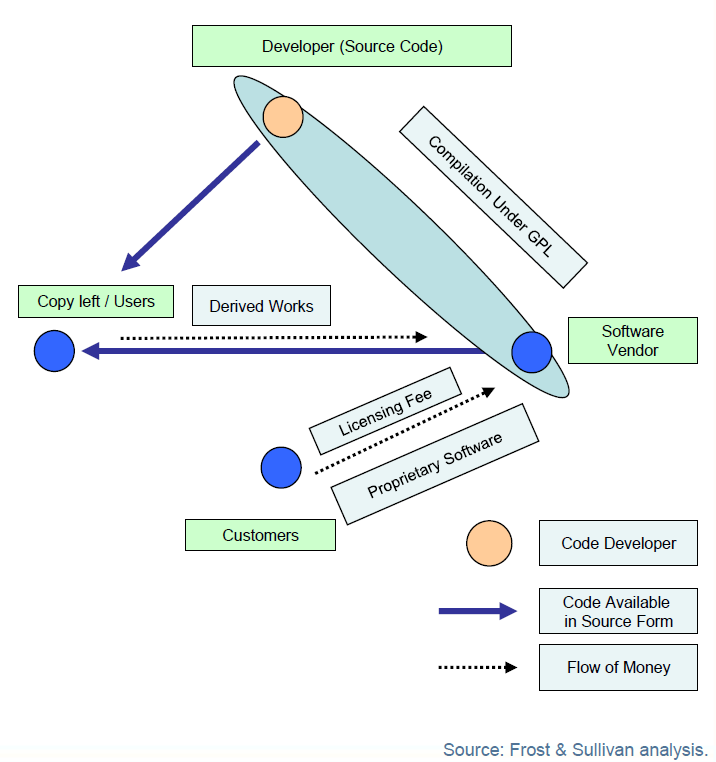
\includegraphics[width=.94\textwidth]{Pictures/Impact-img1.png}


\TODO{An open source architecture allows risk sharing: collaborating
  in the early stages of research could help an early detection, and,
  by consequence, reducing risks.}

\TODO{But: since Open Source softwares are freely accessible, security
  and privacy issues are a concern. Anytime a resource is shared,
  there is greater risk of unauthorised access and contaminated data.
  Providers must demonstrate security solutions, which should include
  physical security controlling access to the facility and protection
  of user data from corruption and cyber attacks.}


%  LocalWords:  mgt Paris-Sud UPSud Thiery Sage-Combinat decentralisation textwidth hline
%  LocalWords:  textwidth Jupyter slmhnlnhfnhs hsfhs ghshsh includegraphics unauthorised
